\documentclass[11pt]{article}

\usepackage[margin=0.85in]{geometry}
\usepackage[T1]{fontenc}
\usepackage[utf8]{inputenc}
\usepackage{lmodern}
\usepackage{amsmath,amssymb,mathtools}
\usepackage{booktabs}
\usepackage{array}
\usepackage{graphicx}
\usepackage{enumitem}
\usepackage{siunitx}
\usepackage{xcolor}
\usepackage{hyperref}
\usepackage{tikz}
\usepackage{pgfplots}
\usepackage{circuitikz}
\usepackage{tcolorbox}
\usepackage{multicol}
\usepackage{longtable}
\usetikzlibrary{arrows.meta,positioning,calc,shapes.geometric,fit}
\pgfplotsset{compat=1.18}

\hypersetup{
  colorlinks=true,
  linkcolor=blue!55!black,
  urlcolor=blue!55!black,
  citecolor=blue!55!black
}

\newcommand{\V}{\mathbf{V}}
\newcommand{\I}{\mathbf{I}}
\newcommand{\Y}{\mathbf{Y}}
\newcommand{\Sbase}{S_{\mathrm{base}}}
\newcommand{\Vbase}{V_{\mathrm{base}}}
\newcommand{\Zbase}{Z_{\mathrm{base}}}
\newcommand{\pu}{\mathrm{pu}}
\newcommand{\dd}{\mathrm{d}}
\newcommand{\junit}{\mathrm{j}}
\newcommand{\Real}{\operatorname{Re}}
\newcommand{\Imag}{\operatorname{Im}}
\newcommand{\highlight}[1]{\textcolor{blue!55!black}{#1}}

\title{\textbf{Power System Study Guide -- Extended Edition}\\
\large From Classical Network Analysis to Inverter-Based Resources, Grid-Forming Control, and Microgrid Fault Ride-Through}
\author{Generated Study Notes}
\date{\today}

\begin{document}
\maketitle

\begin{abstract}
This extended guide summarizes core and advanced power-system topics: per-unit
normalization, bus modeling, power-flow equations, voltage and angle stability,
faults, protection, synchronous-machine dynamics, inverter-based resources
(IBRs), grid-following (GFL) and grid-forming (GFM) controls, the stability
impact of high IBR penetration, and practical ride-through concepts for
microgrids during grid faults. Additional worked details, design checklists,
modeling assumptions, and control/protection notes are included to make the
material useful as both a review sheet and an implementation reference.
\end{abstract}

\tableofcontents
\newpage

\section{Big Picture}

An electric power system converts mechanical, chemical, solar, wind, or stored
energy into electric power, transports it through transmission and distribution
networks, and delivers it to loads with acceptable voltage, frequency,
reliability, power quality, and safety. The traditional grid is dominated by
synchronous generators. Modern grids increasingly include inverter-based
resources such as wind, solar photovoltaic (PV), battery energy storage systems
(BESS), and power-electronic loads.

\begin{figure}[h]
\centering
\resizebox{0.95\linewidth}{!}{%
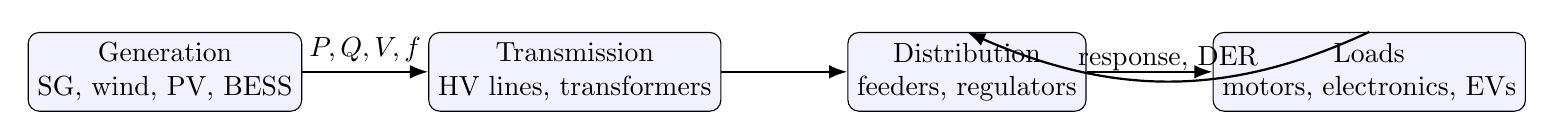
\begin{tikzpicture}[node distance=1.6cm,>=Latex]
  \tikzstyle{block}=[draw,rounded corners,align=center,minimum width=2.6cm,minimum height=1.0cm,fill=blue!5]
  \node[block] (gen) {Generation\\SG, wind, PV, BESS};
  \node[block,right=of gen] (tx) {Transmission\\HV lines, transformers};
  \node[block,right=of tx] (dist) {Distribution\\feeders, regulators};
  \node[block,right=of dist] (load) {Loads\\motors, electronics, EVs};
  \draw[->,thick] (gen) -- node[above] {$P,Q,V,f$} (tx);
  \draw[->,thick] (tx) -- (dist);
  \draw[->,thick] (dist) -- (load);
  \draw[->,thick,bend left=25] (load.north) to node[above] {response, DER} (dist.north);
\end{tikzpicture}
}
\caption{A power system is a controlled energy-conversion network.}
\end{figure}

\section{Phasors, Complex Power, and Per-Unit}

\subsection{Sinusoidal Steady State}
For a sinusoidal voltage,
\begin{equation}
v(t)=\sqrt{2}V_{\mathrm{rms}}\cos(\omega t+\theta),
\end{equation}
the phasor is
\begin{equation}
\tilde{V}=V_{\mathrm{rms}}\angle\theta.
\end{equation}
For balanced three-phase systems, a single-phase equivalent is commonly used.
Line-to-line and phase quantities obey
\begin{equation}
V_{LL}=\sqrt{3}V_{\phi}, \qquad S_{3\phi}=\sqrt{3}V_{LL}I_L.
\end{equation}

\subsection{Complex Power}
Complex power is
\begin{equation}
\tilde{S}=P+\junit Q=\tilde{V}\tilde{I}^{*},
\end{equation}
where $P$ is real power and $Q$ is reactive power. The power factor is
\begin{equation}
\mathrm{pf}=\cos\phi=\frac{P}{|\tilde{S}|}.
\end{equation}
For inductive loads, current lags voltage and $Q>0$ under the usual load sign
convention.

\subsection{Per-Unit System}
Per-unit quantities reduce transformer-ratio bookkeeping and put impedances on
a comparable scale:
\begin{equation}
X_{\pu}=\frac{X_{\mathrm{actual}}}{X_{\mathrm{base}}}.
\end{equation}
For a three-phase base,
\begin{equation}
Z_{\mathrm{base}}=\frac{V_{LL,\mathrm{base}}^2}{S_{3\phi,\mathrm{base}}},
\qquad
I_{\mathrm{base}}=\frac{S_{3\phi,\mathrm{base}}}{\sqrt{3}V_{LL,\mathrm{base}}}.
\end{equation}
Changing base:
\begin{equation}
Z_{\pu,\mathrm{new}}=Z_{\pu,\mathrm{old}}
\left(\frac{S_{\mathrm{base,new}}}{S_{\mathrm{base,old}}}\right)
\left(\frac{V_{\mathrm{base,old}}}{V_{\mathrm{base,new}}}\right)^2.
\end{equation}

\section{Network Modeling}

\subsection{Transmission-Line Models}
For a short line, shunt capacitance can often be neglected:
\begin{equation}
\tilde{V}_S=\tilde{V}_R+\tilde{I}(R+\junit X).
\end{equation}
For medium and long lines, the nominal-$\pi$ model includes shunt admittance
$Y/2$ at both ends.

\begin{figure}[h]
\centering
\begin{circuitikz}[american]
\draw (0,0) to[short,o-] (1,0)
      to[R=$R$, -*] (3,0)
      to[L=$X/\omega$, -*] (5,0)
      to[short,-o] (6,0);
\draw (1,0) to[C,l_=$Y/2\omega$] (1,-2) node[ground]{};
\draw (5,0) to[C,l=$Y/2\omega$] (5,-2) node[ground]{};
\node at (0,0.35) {$V_S$};
\node at (6,0.35) {$V_R$};
\end{circuitikz}
\caption{Nominal-$\pi$ transmission-line model.}
\end{figure}

\subsection{Admittance Matrix}
Nodal current injection satisfies
\begin{equation}
\I=\Y_{\mathrm{bus}}\V.
\end{equation}
For a branch between buses $i$ and $k$ with series admittance $y_{ik}$:
\begin{align}
Y_{ii} &\leftarrow Y_{ii}+y_{ik}+y_{\mathrm{sh},i},\\
Y_{kk} &\leftarrow Y_{kk}+y_{ik}+y_{\mathrm{sh},k},\\
Y_{ik} &=Y_{ki}\leftarrow -y_{ik}.
\end{align}
Transformer off-nominal tap ratios and phase shifters modify these entries and
must be modeled carefully in power-flow and short-circuit studies.

\section{Bus Types: Slack, PV, and PQ}

Power-flow analysis classifies buses by which variables are specified and which
are solved.

\begin{table}[h]
\centering
\begin{tabular}{llll}
\toprule
Bus type & Known quantities & Unknown quantities & Typical device \\
\midrule
Slack / swing & $|V|,\delta$ & $P,Q$ & Reference generator \\
PV / generator & $P,|V|$ & $Q,\delta$ & Generator with AVR \\
PQ / load & $P,Q$ & $|V|,\delta$ & Load or fixed-power DER \\
\bottomrule
\end{tabular}
\caption{Power-flow bus types.}
\end{table}

\begin{itemize}
  \item \textbf{Slack bus:} supplies the real and reactive mismatch after all
  other injections and losses are determined. It sets the system angle reference.
  \item \textbf{PV bus:} real power and voltage magnitude are specified. Reactive
  output is solved, but if it violates limits, the bus is typically converted to
  PQ with $Q$ fixed at the limit.
  \item \textbf{PQ bus:} real and reactive powers are specified. Voltage magnitude
  and angle are solved.
\end{itemize}

\begin{figure}[h]
\centering
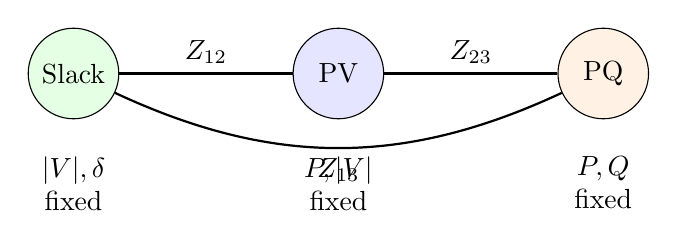
\begin{tikzpicture}[node distance=2.2cm,>=Latex]
  \node[draw,circle,fill=green!10,minimum size=1.15cm] (slack) {Slack};
  \node[draw,circle,fill=blue!10,minimum size=1.15cm,right=of slack] (pv) {PV};
  \node[draw,circle,fill=orange!10,minimum size=1.15cm,right=of pv] (pq) {PQ};
  \draw[thick] (slack) -- node[above] {$Z_{12}$} (pv);
  \draw[thick] (pv) -- node[above] {$Z_{23}$} (pq);
  \draw[thick,bend right=25] (slack) to node[below] {$Z_{13}$} (pq);
  \node[below=0.35cm of slack,align=center] {$|V|,\delta$\\fixed};
  \node[below=0.35cm of pv,align=center] {$P,|V|$\\fixed};
  \node[below=0.35cm of pq,align=center] {$P,Q$\\fixed};
\end{tikzpicture}
\caption{Three classical power-flow bus types.}
\end{figure}

\section{AC Power Flow}

\subsection{Power Injection Equations}
Let $V_i=|V_i|\angle\delta_i$ and
$Y_{ik}=G_{ik}+\junit B_{ik}$. The complex power injected at bus $i$ is
\begin{equation}
S_i=P_i+\junit Q_i=V_i I_i^*=V_i\left(\sum_{k=1}^{n}Y_{ik}V_k\right)^*.
\end{equation}
The real and reactive power equations are
\begin{align}
P_i &= |V_i|\sum_{k=1}^{n}|V_k|
\left(G_{ik}\cos\delta_{ik}+B_{ik}\sin\delta_{ik}\right),\\
Q_i &= |V_i|\sum_{k=1}^{n}|V_k|
\left(G_{ik}\sin\delta_{ik}-B_{ik}\cos\delta_{ik}\right),
\end{align}
where $\delta_{ik}=\delta_i-\delta_k$.

\subsection{Newton--Raphson Method}
Define mismatch vector
\begin{equation}
\Delta x=
\begin{bmatrix}
\Delta P\\
\Delta Q
\end{bmatrix}
=
\begin{bmatrix}
P_{\mathrm{spec}}-P_{\mathrm{calc}}\\
Q_{\mathrm{spec}}-Q_{\mathrm{calc}}
\end{bmatrix}.
\end{equation}
At iteration $r$,
\begin{equation}
\begin{bmatrix}
\Delta P\\
\Delta Q
\end{bmatrix}^{(r)}
=
\begin{bmatrix}
H & N\\
M & L
\end{bmatrix}^{(r)}
\begin{bmatrix}
\Delta \delta\\
\Delta |V|
\end{bmatrix}^{(r)}.
\end{equation}
Update angles and magnitudes until the maximum mismatch is below tolerance.

\subsection{Fast Decoupled Power Flow}
For high-voltage transmission systems, $X\gg R$, voltage magnitudes are near
1 pu, and angle differences are small. Then active power is strongly coupled to
angle and reactive power to voltage:
\begin{align}
\Delta P/|V| &\approx B'\Delta \delta,\\
\Delta Q/|V| &\approx B''\Delta |V|.
\end{align}

\section{Economic Dispatch and Optimal Power Flow}

\subsection{Economic Dispatch}
For generator cost
\begin{equation}
C_i(P_i)=a_iP_i^2+b_iP_i+c_i,
\end{equation}
economic dispatch without losses solves
\begin{equation}
\min_{P_i}\sum_i C_i(P_i)
\quad \text{s.t.}\quad
\sum_i P_i=P_D.
\end{equation}
The optimality condition is
\begin{equation}
\frac{\dd C_i}{\dd P_i}=2a_iP_i+b_i=\lambda,
\end{equation}
subject to generator limits.

\subsection{AC Optimal Power Flow}
AC OPF extends power flow by optimizing an objective subject to network
constraints:
\begin{align}
\min_{V,\delta,P_G,Q_G} \quad & f(P_G,Q_G,V)\\
\text{s.t.}\quad & g(V,\delta,P_G,Q_G)=0,\\
& h(V,\delta,P_G,Q_G)\le 0.
\end{align}
Constraints include bus voltage limits, branch thermal limits, generator
capability curves, reserve requirements, and security constraints.

\section{Short-Circuit and Fault Analysis}

\subsection{Symmetrical Components}
Unbalanced three-phase quantities can be decomposed into positive, negative,
and zero sequences:
\begin{equation}
\begin{bmatrix}V_a\\V_b\\V_c\end{bmatrix}
=
\begin{bmatrix}
1&1&1\\
1&a^2&a\\
1&a&a^2
\end{bmatrix}
\begin{bmatrix}V_0\\V_1\\V_2\end{bmatrix},
\qquad
a=e^{\junit 2\pi/3}.
\end{equation}
The inverse transform is
\begin{equation}
\begin{bmatrix}V_0\\V_1\\V_2\end{bmatrix}
=\frac{1}{3}
\begin{bmatrix}
1&1&1\\
1&a&a^2\\
1&a^2&a
\end{bmatrix}
\begin{bmatrix}V_a\\V_b\\V_c\end{bmatrix}.
\end{equation}

\subsection{Three-Phase Fault}
For a bolted balanced three-phase fault at a bus with Thevenin voltage
$V_{\mathrm{th}}$ and Thevenin impedance $Z_1$,
\begin{equation}
I_f=\frac{V_{\mathrm{th}}}{Z_1+Z_f}.
\end{equation}

\subsection{Single-Line-to-Ground Fault}
For an $a$-phase-to-ground fault:
\begin{equation}
I_a=3I_0=\frac{3V_{\mathrm{th}}}{Z_1+Z_2+Z_0+3Z_f}.
\end{equation}
Grounding and transformer connections strongly affect $Z_0$ and therefore
ground-fault current.

\subsection{Fault Current From Synchronous Machines and IBRs}
Synchronous generators can contribute large transient currents, often several
per-unit initially, limited by subtransient reactance:
\begin{equation}
I_{\mathrm{sc,SG}}\approx \frac{E''}{X''_d}.
\end{equation}
IBRs are current-limited by semiconductors and controls, commonly around
$1.1$--$2.0$ pu depending on design and grid code:
\begin{equation}
|\tilde{I}_{\mathrm{IBR}}|\le I_{\max}.
\end{equation}
This changes protection sensitivity, directionality, relay coordination, and
fault-location methods.

\section{Protection Fundamentals}

Protection detects abnormal conditions and isolates faulted equipment quickly.
Common functions include:
\begin{itemize}
  \item \textbf{50/51 overcurrent:} instantaneous/time-delayed current pickup.
  \item \textbf{67 directional overcurrent:} uses voltage polarization to infer
  fault direction.
  \item \textbf{21 distance:} estimates apparent impedance $Z_{\mathrm{app}}=V/I$.
  \item \textbf{87 differential:} compares currents entering and leaving a zone.
  \item \textbf{27/59 undervoltage/overvoltage} and \textbf{81U/O frequency}
  functions.
  \item \textbf{ROCOF:} rate-of-change-of-frequency, $\dd f/\dd t$.
\end{itemize}

\begin{tcolorbox}[colback=yellow!6,colframe=yellow!45!black,title=IBR Protection Challenge]
High IBR penetration reduces short-circuit current magnitude, changes current
phase angle through control actions, and can make conventional overcurrent
protection less dependable. Protection may need adaptive settings, negative-
sequence quantities, differential schemes, transfer trip, traveling waves, or
communications-assisted logic.
\end{tcolorbox}

\section{Voltage Control and Reactive Power}

\subsection{Reactive Power and Voltage}
In transmission networks with $X\gg R$, reactive power strongly affects voltage.
A useful approximate relation is
\begin{equation}
\Delta V\approx \frac{XQ+RP}{V}.
\end{equation}
Devices for voltage support include generator automatic voltage regulators
(AVRs), shunt capacitors/reactors, static VAR compensators (SVC), STATCOMs,
load tap changers, and inverter volt-var controls.

\subsection{Generator Capability}
Synchronous-generator reactive power is limited by armature current, field
current, end-region heating, and stability. IBR reactive capability is limited
by current and dc-link constraints:
\begin{equation}
P^2+Q^2\le S_{\mathrm{rated}}^2, \qquad
I_d^2+I_q^2\le I_{\max}^2.
\end{equation}
During faults, priority may be given to reactive current injection:
\begin{equation}
I_q^{*}=k_{\mathrm{FRT}}\left(V_{\mathrm{ref}}-V_{\mathrm{PCC}}\right),
\qquad |I^*|\le I_{\max}.
\end{equation}

\section{Frequency Control and Inertia}

\subsection{Swing Equation}
The synchronous-machine rotor angle follows
\begin{equation}
M\frac{\dd^2\delta}{\dd t^2}=P_m-P_e-D\frac{\dd \delta}{\dd t},
\end{equation}
or, in frequency form,
\begin{equation}
\frac{2H}{f_0}\frac{\dd f}{\dd t}=P_m-P_e-D_f(f-f_0),
\end{equation}
where $H$ is the inertia constant. Immediately after a generation-loss event,
frequency rate of change is approximately
\begin{equation}
\frac{\dd f}{\dd t}\approx \frac{f_0}{2H_{\mathrm{sys}}}
\left(\frac{\Delta P}{S_{\mathrm{base}}}\right).
\end{equation}

\subsection{Primary, Secondary, and Tertiary Control}
\begin{itemize}
  \item \textbf{Primary control:} governor or inverter droop responds in seconds.
  \item \textbf{Secondary control:} automatic generation control restores
  frequency and tie-line interchange in tens of seconds to minutes.
  \item \textbf{Tertiary control:} economic redispatch and reserve management.
\end{itemize}

\section{Stability Concepts}

\subsection{Rotor-Angle Stability}
Rotor-angle stability is the ability of synchronous machines to remain in
synchronism. For a classical generator connected to an infinite bus:
\begin{equation}
P_e=\frac{EV}{X}\sin\delta.
\end{equation}
The synchronizing torque coefficient is
\begin{equation}
K_s=\frac{\partial P_e}{\partial \delta}=\frac{EV}{X}\cos\delta.
\end{equation}
As $\delta$ approaches \SI{90}{\degree}, synchronizing torque decreases.

\subsection{Equal-Area Criterion}
For a single-machine infinite-bus system, transient stability can be assessed by
comparing accelerating and decelerating areas on the $P$--$\delta$ curve:
\begin{equation}
A_{\mathrm{acc}}=\int_{\delta_0}^{\delta_c}(P_m-P_{e,\mathrm{fault}})\,\dd\delta,
\qquad
A_{\mathrm{dec}}=\int_{\delta_c}^{\delta_{\max}}(P_{e,\mathrm{post}}-P_m)\,\dd\delta.
\end{equation}
Stability requires $A_{\mathrm{dec}}\ge A_{\mathrm{acc}}$.

\subsection{Voltage Stability}
Voltage stability is the ability to maintain acceptable voltage after a
disturbance. A simple radial two-bus example shows the ``nose curve'':

\begin{figure}[h]
\centering
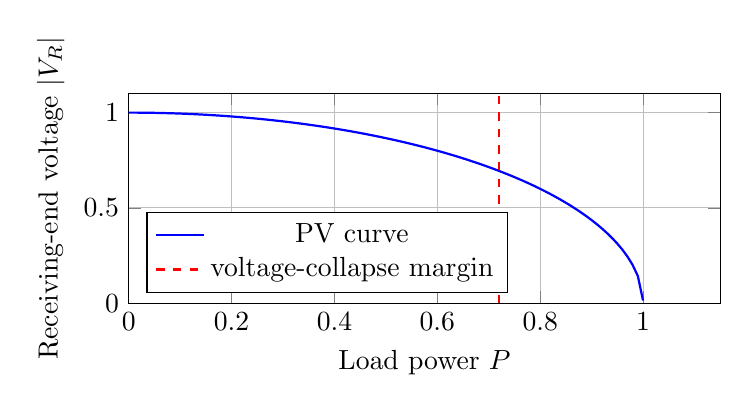
\begin{tikzpicture}
\begin{axis}[
  width=0.75\linewidth,
  height=0.35\linewidth,
  xlabel={Load power $P$},
  ylabel={Receiving-end voltage $|V_R|$},
  xmin=0,xmax=1.15,ymin=0,ymax=1.1,
  grid=both,
  domain=0:1,
  samples=100,
  legend style={at={(0.03,0.05)},anchor=south west}
]
\addplot[blue,thick] ({x},{sqrt(max(0,1-x^2))});
\addplot[red,dashed,thick] coordinates {(0.72,0) (0.72,1.1)};
\legend{PV curve, voltage-collapse margin}
\end{axis}
\end{tikzpicture}
\caption{Conceptual PV curve showing maximum loadability and voltage-collapse margin.}
\end{figure}

\subsection{Small-Signal Stability}
Linearize nonlinear dynamics $\dot{x}=f(x,u)$ around an operating point:
\begin{equation}
\Delta \dot{x}=A\Delta x+B\Delta u.
\end{equation}
Eigenvalues $\lambda_i=\sigma_i+\junit \omega_i$ determine modal behavior.
The damping ratio is
\begin{equation}
\zeta_i=\frac{-\sigma_i}{\sqrt{\sigma_i^2+\omega_i^2}}.
\end{equation}
Negative damping or weak inter-area modes can be worsened by controls that
interact with grid impedance, PLLs, or other converters.

\section{Power Quality}

Power quality includes voltage sags, swells, interruptions, harmonics, flicker,
unbalance, and transients. Harmonic distortion is quantified by
\begin{equation}
\mathrm{THD}_V=\frac{\sqrt{V_2^2+V_3^2+\cdots+V_n^2}}{V_1}.
\end{equation}
Converters use filters and controls to meet harmonic limits. Resonance can occur
when inverter filters, cable capacitance, transformer leakage, and grid
impedance form lightly damped modes.

\section{Inverter-Based Resources}

\subsection{What Is an IBR?}
An IBR interfaces an energy source or storage device through power electronics.
Examples include PV inverters, wind turbine full converters, type-3 wind
generators with partial converters, BESS, fuel cells, and many HVDC terminals.

\subsection{Converter Power Equations in \texorpdfstring{$dq$}{dq} Coordinates}
With the $d$-axis aligned to voltage, $v_q=0$:
\begin{align}
P &= \frac{3}{2}(v_di_d+v_qi_q)=\frac{3}{2}v_di_d,\\
Q &= \frac{3}{2}(v_qi_d-v_di_q)=-\frac{3}{2}v_di_q.
\end{align}
Thus $i_d$ controls active power and $i_q$ controls reactive power under this
axis convention.

\subsection{Grid-Following (GFL) Inverters}
A GFL inverter behaves like a controlled current source. It synchronizes to an
existing grid voltage using a phase-locked loop (PLL), then injects commanded
currents.

\begin{figure}[h]
\centering
\resizebox{0.95\linewidth}{!}{%
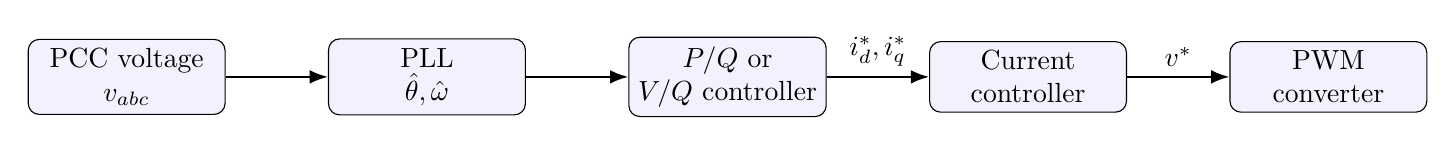
\begin{tikzpicture}[>=Latex,node distance=1.3cm]
  \tikzstyle{block}=[draw,rounded corners,align=center,minimum width=2.5cm,minimum height=0.8cm,fill=blue!5]
  \node[block] (pcc) {PCC voltage\\$v_{abc}$};
  \node[block,right=of pcc] (pll) {PLL\\$\hat{\theta},\hat{\omega}$};
  \node[block,right=of pll] (pq) {$P/Q$ or\\$V/Q$ controller};
  \node[block,right=of pq] (curr) {Current\\controller};
  \node[block,right=of curr] (pwm) {PWM\\converter};
  \draw[->,thick] (pcc) -- (pll);
  \draw[->,thick] (pll) -- (pq);
  \draw[->,thick] (pq) -- node[above] {$i_d^*,i_q^*$} (curr);
  \draw[->,thick] (curr) -- node[above] {$v^*$} (pwm);
\end{tikzpicture}
}
\caption{Grid-following inverter control is synchronized by the measured grid voltage.}
\end{figure}

Typical GFL PLL dynamics include
\begin{equation}
\dot{\hat{\theta}}=\omega_0+K_p v_q+K_i\int v_q\,\dd t.
\end{equation}
GFL inverters are effective in strong grids but can struggle in weak grids or
islanded microgrids because they require a voltage reference to follow.

\subsection{Grid-Forming (GFM) Inverters}
A GFM inverter behaves more like a controllable voltage source behind an
impedance. It establishes voltage magnitude and frequency rather than relying
entirely on an external voltage.

Common GFM approaches:
\begin{itemize}
  \item \textbf{Droop control:}
  \begin{align}
  \omega &= \omega_0-m_p(P-P_0),\\
  V &= V_0-n_q(Q-Q_0).
  \end{align}
  \item \textbf{Virtual synchronous machine (VSM):}
  \begin{equation}
  2H_{\mathrm{v}}\dot{\omega}=P^{*}-P-D_{\mathrm{v}}(\omega-\omega_0).
  \end{equation}
  \item \textbf{Dispatchable virtual oscillator control:} nonlinear oscillator
  dynamics regulate voltage waveform and share power.
  \item \textbf{Matching control:} uses dc-link dynamics to emulate
  synchronous-machine electromechanical coupling.
\end{itemize}

\begin{figure}[h]
\centering
\resizebox{0.95\linewidth}{!}{%
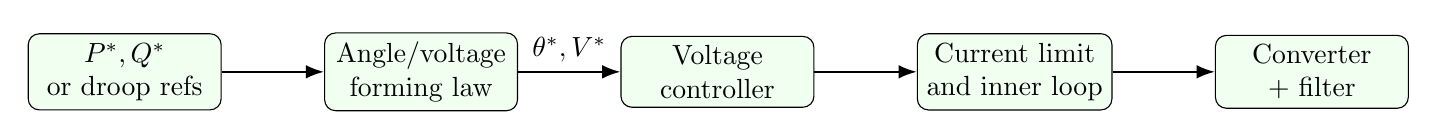
\begin{tikzpicture}[>=Latex,node distance=1.3cm]
  \tikzstyle{block}=[draw,rounded corners,align=center,minimum width=2.45cm,minimum height=0.8cm,fill=green!6]
  \node[block] (pref) {$P^*,Q^*$\\or droop refs};
  \node[block,right=of pref] (osc) {Angle/voltage\\forming law};
  \node[block,right=of osc] (volt) {Voltage\\controller};
  \node[block,right=of volt] (curr) {Current limit\\and inner loop};
  \node[block,right=of curr] (conv) {Converter\\+ filter};
  \draw[->,thick] (pref) -- (osc);
  \draw[->,thick] (osc) -- node[above] {$\theta^*,V^*$} (volt);
  \draw[->,thick] (volt) -- (curr);
  \draw[->,thick] (curr) -- (conv);
\end{tikzpicture}
}
\caption{Grid-forming inverter control creates a voltage/frequency reference.}
\end{figure}

\subsection{GFL vs GFM Summary}
\begin{longtable}{p{0.2\linewidth}p{0.36\linewidth}p{0.36\linewidth}}
\toprule
Feature & Grid-following & Grid-forming \\
\midrule
Equivalent behavior & Current source & Voltage source behind impedance \\
Synchronization & PLL follows grid voltage & Internal oscillator or swing-like law \\
Islanded operation & Not sufficient alone & Can support islanded microgrid \\
Weak-grid performance & PLL/control interactions possible & Can improve voltage/frequency stiffness \\
Fault response & Current-limited injection & Must handle current limiting without losing voltage-forming behavior \\
Power sharing & Usually outer-loop command & Droop/VSM sharing natural \\
\bottomrule
\end{longtable}

\section{How IBRs Affect Power-Grid Stability}

\subsection{Reduced Inertia and Faster Dynamics}
Replacing synchronous machines with IBRs reduces physical rotating inertia unless
the IBR control intentionally provides synthetic inertia or fast frequency
response. Lower inertia produces higher ROCOF:
\begin{equation}
\left|\frac{\dd f}{\dd t}\right|\propto \frac{|\Delta P|}{H_{\mathrm{sys}}}.
\end{equation}
However, IBRs can respond much faster than mechanical governors if controls,
energy headroom, and communications are designed correctly.

\subsection{PLL and Weak-Grid Instability}
Grid strength is often measured using short-circuit ratio:
\begin{equation}
\mathrm{SCR}=\frac{S_{\mathrm{sc}}}{S_{\mathrm{IBR,rated}}},
\qquad
S_{\mathrm{sc}}=\frac{V^2}{|Z_{\mathrm{th}}|}.
\end{equation}
Low SCR means the inverter's own current injection significantly moves the PCC
voltage. For GFL controls, PLL dynamics can couple with the weak grid and create
oscillations. Effective grid strength can also be reduced by nearby converters
interacting through the same network.

\subsection{Current Limiting and Protection}
IBRs cannot supply unlimited fault current. During severe voltage depressions,
the current limit
\begin{equation}
\sqrt{i_d^2+i_q^2}\le I_{\max}
\end{equation}
forces a choice between active current, reactive support, negative-sequence
current, and dc-link protection. This affects voltage recovery, relay
dependability, and transient stability.

\subsection{Control Interactions}
High IBR penetration introduces many fast controls: PLLs, current loops, dc-link
loops, volt-var controls, plant-level controllers, and grid-forming controllers.
Interactions can occur over milliseconds to seconds. Stability studies must
include electromagnetic transient (EMT) simulations for fast converter controls
when RMS phasor models are insufficient.

\subsection{Fault-Induced Delayed Voltage Recovery}
IBRs often ride through voltage sags and inject reactive current, but motor loads,
feeder controls, and current-limited converters may cause slow voltage recovery.
Coordination among DER ride-through, distribution protection, and transmission
voltage controls is essential.

\section{Microgrids}

\subsection{Definition and Modes}
A microgrid is a local system of loads, DERs, storage, protection, and controls
that can operate grid-connected or islanded. It needs:
\begin{itemize}
  \item at least one grid-forming source for islanded voltage/frequency,
  \item energy management for power balance,
  \item protection that works for both grid-connected and islanded fault levels,
  \item black-start and resynchronization procedures.
\end{itemize}

\subsection{Microgrid Control Hierarchy}
\begin{enumerate}
  \item \textbf{Primary control:} local voltage/frequency regulation, droop,
  current limiting, and virtual impedance.
  \item \textbf{Secondary control:} restores frequency/voltage deviations caused
  by droop and coordinates multiple DERs.
  \item \textbf{Tertiary control:} economic dispatch and power exchange with the
  main grid.
\end{enumerate}

\begin{figure}[h]
\centering
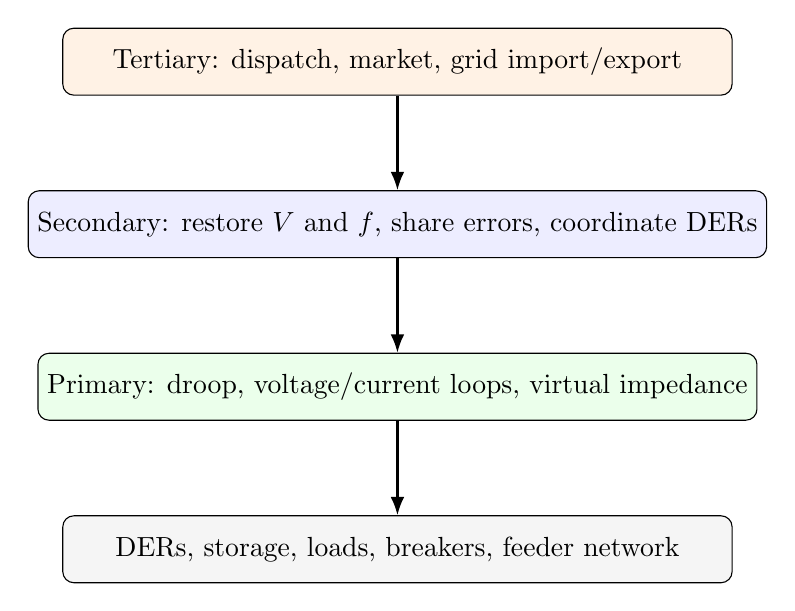
\begin{tikzpicture}[>=Latex,node distance=1.2cm]
  \tikzstyle{layer}=[draw,rounded corners,align=center,minimum width=8.5cm,minimum height=0.85cm]
  \node[layer,fill=green!8] (primary) {Primary: droop, voltage/current loops, virtual impedance};
  \node[layer,fill=blue!7,above=of primary] (secondary) {Secondary: restore $V$ and $f$, share errors, coordinate DERs};
  \node[layer,fill=orange!10,above=of secondary] (tertiary) {Tertiary: dispatch, market, grid import/export};
  \draw[->,thick] (tertiary) -- (secondary);
  \draw[->,thick] (secondary) -- (primary);
  \node[draw,rounded corners,fill=gray!8,below=of primary,minimum width=8.5cm,minimum height=0.85cm,align=center] (plant)
  {DERs, storage, loads, breakers, feeder network};
  \draw[->,thick] (primary) -- (plant);
\end{tikzpicture}
\caption{Microgrid hierarchical control.}
\end{figure}

\section{Ride-Through During Faults}

\subsection{Meaning of Ride-Through}
Ride-through means that DERs remain connected and support the grid or microgrid
during abnormal voltage/frequency events instead of tripping immediately.
Requirements are usually defined by voltage--time and frequency--time envelopes.

\begin{figure}[h]
\centering
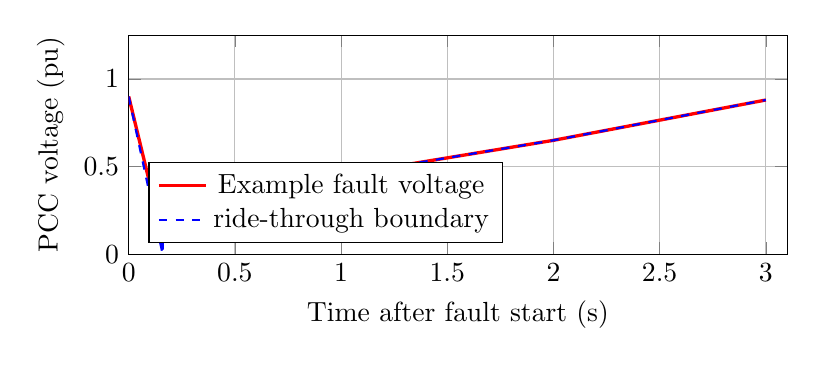
\begin{tikzpicture}
\begin{axis}[
  width=0.82\linewidth,
  height=0.36\linewidth,
  xlabel={Time after fault start (s)},
  ylabel={PCC voltage (pu)},
  xmin=0,xmax=3.1,ymin=0,ymax=1.25,
  grid=both,
  legend style={at={(0.03,0.05)},anchor=south west}
]
\addplot[red,very thick] coordinates {(0,0.9) (0.15,0.15) (0.625,0.15) (1.0,0.45) (2.0,0.65) (3.0,0.88)};
\addplot[blue,dashed,thick] coordinates {(0,0.9) (0.16,0.0) (0.16,0.45) (1.0,0.45) (2.0,0.65) (3.0,0.88)};
\legend{Example fault voltage, ride-through boundary}
\end{axis}
\end{tikzpicture}
\caption{Conceptual low-voltage ride-through envelope. Actual limits depend on grid code.}
\end{figure}

\subsection{Core Ride-Through Mechanisms}
Fault ride-through for an inverter-dominated microgrid usually combines:
\begin{enumerate}
  \item \textbf{Fast fault detection:} voltage sag, current rise, negative/zero
  sequence, impedance, or differential signals.
  \item \textbf{Current limiting:} protects semiconductors and filters while
  maintaining a controlled current vector.
  \item \textbf{Reactive current priority:} supports voltage at the PCC during
  low-voltage events.
  \item \textbf{Active power reduction:} prevents dc-link overvoltage when ac
  power export is limited by sagged voltage.
  \item \textbf{Energy buffering:} BESS, dc-link capacitance, braking chopper, or
  curtailment absorbs mismatch.
  \item \textbf{Protection coordination:} isolates only the faulted zone.
  \item \textbf{Post-fault recovery:} ramps current, voltage, and power references
  to avoid secondary dips or converter interactions.
\end{enumerate}

\subsection{Current-Limited Control During a Fault}
Let $I_{\max}$ be the converter current limit. A common current-priority logic is
\begin{align}
i_q^{*} &= \operatorname{sat}\left(k_v(V_{\mathrm{ref}}-V_{\mathrm{PCC}}),
 -I_{\max}, I_{\max}\right),\\
i_d^{*} &= \operatorname{sgn}(P^{*})
\sqrt{\max\left(I_{\max}^2-(i_q^{*})^2,0\right)}.
\end{align}
If the inverter uses the opposite $dq$ sign convention, the sign of $i_q$ must be
changed. For GFM inverters, the current limit must be integrated without abruptly
collapsing the voltage reference. Common methods are virtual impedance, voltage
reference saturation, current reference limiting, and mode switching to a
protected current-source behavior.

\subsection{GFM Fault Ride-Through}
GFM ride-through is difficult because a voltage source behind low impedance would
naturally produce very high fault current. Practical GFM controls add a virtual
impedance:
\begin{equation}
v_{\mathrm{cmd}}=v_{\mathrm{gfm}}-R_v i-L_v\frac{\dd i}{\dd t},
\end{equation}
or reduce voltage reference when current approaches the limit:
\begin{equation}
V^{*}_{\mathrm{lim}}=V^{*}\min\left(1,\frac{I_{\max}}{|I|}\right).
\end{equation}
After clearing, the controller restores normal voltage-forming behavior with
rate limits:
\begin{equation}
\left|\frac{\dd P^{*}}{\dd t}\right|\le r_P,\qquad
\left|\frac{\dd V^{*}}{\dd t}\right|\le r_V.
\end{equation}

\subsection{Microgrid Fault-Ride-Through Sequence}
\begin{figure}[h]
\centering
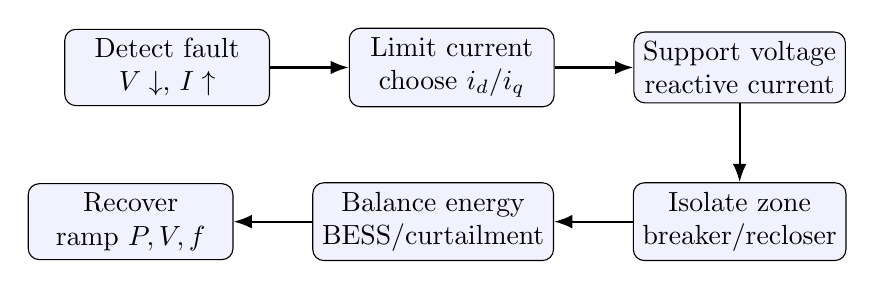
\begin{tikzpicture}[>=Latex,node distance=1.0cm]
  \tikzstyle{rtstep}=[draw,rounded corners,align=center,minimum width=2.6cm,minimum height=0.8cm,fill=blue!5]
  \node[rtstep] (detect) {Detect fault\\$V\downarrow$, $I\uparrow$};
  \node[rtstep,right=of detect] (limit) {Limit current\\choose $i_d/i_q$};
  \node[rtstep,right=of limit] (support) {Support voltage\\reactive current};
  \node[rtstep,below=of support] (isolate) {Isolate zone\\breaker/recloser};
  \node[rtstep,left=of isolate] (balance) {Balance energy\\BESS/curtailment};
  \node[rtstep,left=of balance] (recover) {Recover\\ramp $P,V,f$};
  \draw[->,thick] (detect) -- (limit);
  \draw[->,thick] (limit) -- (support);
  \draw[->,thick] (support) -- (isolate);
  \draw[->,thick] (isolate) -- (balance);
  \draw[->,thick] (balance) -- (recover);
\end{tikzpicture}
\caption{A practical sequence for microgrid fault ride-through.}
\end{figure}

\subsection{Islanded Microgrid Faults}
Islanded microgrids have much lower fault current than utility-connected
systems, especially when dominated by IBRs. Protection may use:
\begin{itemize}
  \item differential protection inside critical zones,
  \item directional elements with adaptive settings,
  \item voltage-based and sequence-based detection,
  \item communication-assisted trip,
  \item temporary overcurrent capability from selected grid-forming BESS,
  \item fast solid-state breakers or hybrid breakers.
\end{itemize}
For unbalanced faults, GFM controls may regulate positive sequence while
selectively injecting negative-sequence current:
\begin{equation}
\begin{bmatrix}i_1^*\\i_2^*\end{bmatrix}
=
\begin{bmatrix}
f_1(V_1,P^*,Q^*)\\
f_2(V_2,I_{\max})
\end{bmatrix},
\qquad |i_1^*+i_2^*|\le I_{\max}.
\end{equation}

\section{EMT and DER}

\subsection{Why EMT Studies Matter for DER-Rich Grids}
Electromagnetic transient (EMT) simulation solves instantaneous voltages and
currents rather than only positive-sequence phasors. This is important for
distributed energy resources (DERs) because converter controls, phase-locked
loops, current limiters, dc-link dynamics, filters, and protection logic can act
within microseconds to milliseconds. RMS or phasor-domain models are still useful
for large-system electromechanical dynamics, but they may hide fast converter
instability, unbalanced behavior, harmonics, and protection miscoordination.

\begin{tcolorbox}[colback=green!5,colframe=green!45!black,title=When to Use EMT]
Use EMT when the study involves inverter controls, weak grids, low short-circuit
ratio, unbalanced faults, fast ride-through behavior, harmonics, resonance,
sub-cycle protection, islanded microgrids, black start, or detailed switching.
\end{tcolorbox}

The basic network equations in EMT are differential equations in physical time:
\begin{align}
v_L(t)&=L\frac{\dd i_L(t)}{\dd t},\\
i_C(t)&=C\frac{\dd v_C(t)}{\dd t},\\
v_R(t)&=Ri_R(t).
\end{align}
Numerical integration converts these equations into discrete-time companion
models. If the EMT time step is $\Delta t$, it must be small enough to represent
the fastest control, switching, and network modes of interest.

\subsection{DER Types and EMT Modeling Blocks}
DERs include rooftop PV, utility-scale PV connected at distribution voltages,
BESS, wind, fuel cells, microturbines, electric vehicles, and controllable
loads. A detailed EMT DER model commonly contains:
\begin{itemize}
  \item dc source or machine-side model,
  \item dc-link capacitor and protection,
  \item voltage-source converter bridge,
  \item pulse-width modulation or averaged converter model,
  \item $L$, $LC$, or $LCL$ filter,
  \item transformer and grounding model,
  \item PLL or grid-forming angle generator,
  \item inner current/voltage loops,
  \item outer active/reactive power, volt-var, volt-watt, and frequency-watt loops,
  \item current limiting and ride-through state machines,
  \item plant controller and communication delays where relevant.
\end{itemize}

\begin{figure}[h]
\centering
\resizebox{0.95\linewidth}{!}{%
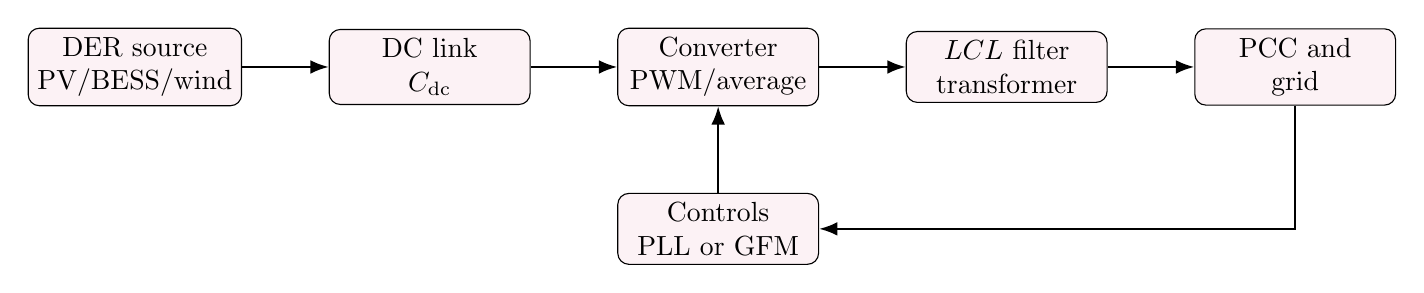
\begin{tikzpicture}[>=Latex,node distance=1.1cm]
  \tikzstyle{derblock}=[draw,rounded corners,align=center,minimum width=2.55cm,minimum height=0.8cm,fill=purple!5]
  \node[derblock] (source) {DER source\\PV/BESS/wind};
  \node[derblock,right=of source] (dc) {DC link\\$C_{\mathrm{dc}}$};
  \node[derblock,right=of dc] (conv) {Converter\\PWM/average};
  \node[derblock,right=of conv] (filter) {$LCL$ filter\\transformer};
  \node[derblock,right=of filter] (grid) {PCC and\\grid};
  \node[derblock,below=of conv] (ctrl) {Controls\\PLL or GFM};
  \draw[->,thick] (source) -- (dc);
  \draw[->,thick] (dc) -- (conv);
  \draw[->,thick] (conv) -- (filter);
  \draw[->,thick] (filter) -- (grid);
  \draw[->,thick] (grid.south) |- (ctrl.east);
  \draw[->,thick] (ctrl.north) -- (conv.south);
\end{tikzpicture}
}
\caption{Typical EMT modeling blocks for an inverter-interfaced DER.}
\end{figure}

\subsection{Faults and Short-Circuit Currents in DER Systems}
Classical short-circuit analysis assumes fault current is driven by voltage
sources behind impedances. This is often valid for synchronous machines:
\begin{equation}
I_{\mathrm{fault,SG}}\approx \frac{E''}{R_s+\junit X_d''+Z_f}.
\end{equation}
DER inverters behave differently because semiconductor ratings and controls
limit current:
\begin{equation}
|\tilde{I}_{\mathrm{fault,DER}}|\le I_{\max}.
\end{equation}
The current waveform may be controlled to prioritize reactive current, positive
sequence, negative sequence, dc-link protection, or thermal protection. Therefore
fault current magnitude, phase angle, and sequence content are control-dependent.

\paragraph{Protection implication.}
In a DER-rich feeder, the fault current seen by an overcurrent relay can be
lower in islanded mode than in grid-connected mode:
\begin{equation}
I_{\mathrm{fault,grid\ connected}}\gg I_{\mathrm{fault,islanded}}.
\end{equation}
This motivates adaptive settings, differential protection, directional
elements, transfer trip, communication-assisted schemes, or voltage/sequence
logic.

\paragraph{Unbalanced faults.}
For line-to-ground and line-to-line faults, DER controls may suppress or command
negative-sequence current. A current-limited positive/negative-sequence command
must satisfy
\begin{equation}
|i_1^*+i_2^*+i_0^*|\le I_{\max}.
\end{equation}
If a model assumes no negative-sequence current when the real inverter injects
some, relay behavior and voltage unbalance predictions may be wrong.

\subsection{Weak Grids and Short-Circuit Ratio}
Grid strength describes how much the PCC voltage changes when the DER injects
current. A common metric is short-circuit ratio:
\begin{equation}
\mathrm{SCR}=\frac{S_{\mathrm{sc}}}{S_{\mathrm{DER,rated}}}
=\frac{V_{\mathrm{PCC}}^2/|Z_{\mathrm{th}}|}{S_{\mathrm{DER,rated}}}.
\end{equation}
Lower SCR means a weaker grid. In weak grids, the inverter is not merely
responding to the grid voltage; its own current injection significantly changes
that voltage:
\begin{equation}
\Delta V_{\mathrm{PCC}}\approx Z_{\mathrm{th}}\Delta I_{\mathrm{DER}}.
\end{equation}

\begin{center}
\begin{tabular}{ll}
\toprule
SCR range & Typical interpretation \\
\midrule
$\mathrm{SCR}>5$ & Strong grid for many conventional GFL controls \\
$3<\mathrm{SCR}\le 5$ & Moderate grid; controls should be checked \\
$2<\mathrm{SCR}\le 3$ & Weak grid; EMT and control tuning often needed \\
$\mathrm{SCR}\le 2$ & Very weak grid; GFM or special controls may be required \\
\bottomrule
\end{tabular}
\end{center}

For multiple nearby DER plants, weighted short-circuit ratio (WSCR) or
impedance-based methods may be more informative than individual SCR, because
plants interact through the shared network.

\subsection{Low Inertia and Fast DER Frequency Response}
Synchronous-machine inertia naturally resists frequency changes. Inverter-based
DERs do not inherently provide mechanical inertia, so high DER penetration can
increase ROCOF after a disturbance:
\begin{equation}
\frac{\dd f}{\dd t}\approx
\frac{f_0}{2H_{\mathrm{sys}}}\frac{\Delta P}{S_{\mathrm{base}}}.
\end{equation}
DERs can still support frequency through fast frequency response:
\begin{align}
\Delta P_{\mathrm{droop}}&=-K_f(f-f_0),\\
P_{\mathrm{synthetic\ inertia}}&=-K_{\mathrm{in}}\frac{\dd f}{\dd t}.
\end{align}
These controls require available headroom and energy. PV may need curtailment to
increase output after underfrequency. BESS can inject or absorb power rapidly,
but it is limited by state of charge, current rating, and thermal constraints.

\begin{tcolorbox}[colback=yellow!6,colframe=yellow!45!black,title=Low-Inertia Design Issue]
Fast DER response improves frequency nadir only if measurement delay, control
delay, communication delay, and power limits are included. A response that is
too aggressive can excite oscillations in weak grids or microgrids.
\end{tcolorbox}

\subsection{PLL Dynamics and Stability}
A grid-following DER uses a PLL to estimate the grid voltage angle. In the
synchronous reference frame, a simple PLL drives $v_q$ toward zero:
\begin{align}
\dot{\xi}_{\mathrm{PLL}} &= v_q,\\
\hat{\omega} &= \omega_0+K_p v_q+K_i\xi_{\mathrm{PLL}},\\
\dot{\hat{\theta}} &= \hat{\omega}.
\end{align}
In a strong grid, the PCC voltage is nearly unaffected by inverter current, so
the PLL sees a stiff reference. In a weak grid, inverter current changes the PCC
voltage angle and magnitude; the PLL then interacts with the current controller
and grid impedance. This can cause low-frequency oscillations, loss of
synchronism, or false ride-through behavior.

\paragraph{PLL tuning tradeoff.}
A fast PLL tracks angle jumps quickly but is more sensitive to voltage
distortion, unbalance, and weak-grid coupling. A slow PLL filters disturbances
better but may track faults and phase jumps poorly. EMT studies should test
faults, voltage phase-angle jumps, weak-grid dispatch points, and neighboring
converter interactions.

\subsection{IEEE 1547 and DER Interconnection Behavior}
IEEE 1547 defines interconnection and interoperability requirements for DERs
connected to electric power systems. Exact settings depend on the adopted
edition, authority having jurisdiction, utility requirements, DER category, and
application. Important study concepts include:
\begin{itemize}
  \item voltage and frequency ride-through requirements,
  \item mandatory voltage and frequency trip settings,
  \item reactive power capability and voltage regulation modes,
  \item volt-var, volt-watt, frequency-watt, and constant power factor functions,
  \item response to abnormal voltage and frequency,
  \item interoperability and communications,
  \item limitations on unintentional islanding,
  \item power quality requirements such as harmonics and flicker.
\end{itemize}

\paragraph{Common DER grid-support functions.}
Volt-var control adjusts reactive power based on PCC voltage:
\begin{equation}
Q^*=f_{\mathrm{VV}}(V_{\mathrm{PCC}}).
\end{equation}
Volt-watt control reduces active power at high voltage:
\begin{equation}
P^*=f_{\mathrm{VW}}(V_{\mathrm{PCC}}).
\end{equation}
Frequency-watt control changes active power with frequency:
\begin{equation}
P^*=P_0-K_{\mathrm{FW}}(f-f_0).
\end{equation}
These functions can improve grid support, but many DERs responding with similar
curves can interact with feeder voltage regulators, capacitor banks, and each
other.

\subsection{DER Ride-Through in EMT}
During a fault, DER ride-through can be represented as a sequence of control
states:
\begin{enumerate}
  \item detect abnormal voltage, frequency, current, or sequence component,
  \item enter ride-through mode if the event is inside the required envelope,
  \item limit current while prioritizing required support,
  \item manage dc-link energy through curtailment, BESS, or chopper,
  \item avoid nuisance tripping while protecting the converter,
  \item ramp back to normal commands after voltage and frequency recover.
\end{enumerate}
The EMT model should include saturation and limiters because they dominate
behavior during faults:
\begin{align}
i_q^*&=\operatorname{sat}\left(k_v(V_{\mathrm{ref}}-V_{\mathrm{PCC}}),
-I_{\max},I_{\max}\right),\\
i_d^*&=\operatorname{sat}\left(\frac{2P^*}{3v_d},-I_{d,\max},I_{d,\max}\right),\\
\sqrt{(i_d^*)^2+(i_q^*)^2}&\le I_{\max}.
\end{align}
If the grid code gives reactive current priority, $i_q^*$ is assigned first and
the remaining current headroom is used for $i_d^*$.

\subsection{EMT Study Checklist for DER Interconnection}
An EMT DER study should include:
\begin{itemize}
  \item validated DER models for all relevant operating modes,
  \item short-circuit ratio and grid impedance sensitivity,
  \item balanced and unbalanced faults at the PCC and nearby buses,
  \item fault clearing, reclosing, and voltage phase-angle jumps,
  \item IEEE 1547 ride-through and trip settings used by the project,
  \item PLL and current-control bandwidth sensitivity,
  \item harmonic and resonance scans for filters, cables, and capacitor banks,
  \item islanding, black-start, and resynchronization cases for microgrids,
  \item protection dependability and security in grid-connected and islanded modes,
  \item post-fault active-power recovery and voltage recovery performance.
\end{itemize}

\subsection{Related Advanced Topics}
\paragraph{Impedance-based stability.}
Converter-grid oscillations can be assessed by measuring or modeling converter
output impedance and grid impedance. Instability risk increases when impedance
ratios encircle critical points in a Nyquist test:
\begin{equation}
L(s)=Z_{\mathrm{grid}}(s)Y_{\mathrm{converter}}(s).
\end{equation}

\paragraph{Harmonics and resonance.}
An $LCL$ filter resonance frequency is approximately
\begin{equation}
\omega_r=\sqrt{\frac{L_1+L_2}{L_1L_2C_f}}.
\end{equation}
Weak grids shift damping and resonance behavior because the grid impedance is
part of the filter seen by the converter.

\paragraph{EMT model fidelity.}
Switching models capture semiconductor switching and harmonics but require small
time steps. Averaged models are faster and often sufficient for control and
ride-through studies if harmonics and switching transients are not the focus.
The model should be no more detailed than necessary, but detailed enough to
represent the phenomenon being studied.

\section{Advanced Study Methods}

\subsection{RMS Phasor vs EMT Simulation}
\begin{itemize}
  \item \textbf{RMS/transient-stability simulation:} efficient for electromechanical
  dynamics, governor/AVR response, and large systems.
  \item \textbf{EMT simulation:} necessary for converter switching, PLL dynamics,
  unbalanced faults, harmonics, sub-synchronous/control interactions, and
  protection details.
\end{itemize}
High IBR systems often require EMT model validation because average phasor models
may hide fast control instabilities.

\subsection{Impedance-Based Stability}
Converter-grid interactions can be studied using source and load impedances. A
small-signal stability condition can be framed with the minor-loop gain
\begin{equation}
L(s)=Z_{\mathrm{source}}(s)Y_{\mathrm{load}}(s),
\end{equation}
and Nyquist criteria. Weak grids have larger $Z_{\mathrm{source}}$, making
interaction with converter input admittance more likely.

\subsection{Resonance and Sub-Synchronous Oscillation}
Series compensation, wind plants, HVDC, and converter controls can create
oscillations below or above the fundamental frequency. Modal damping,
impedance scans, and EMT studies are used to identify risk.

\section{Extended Topic Details and Worked Examples}

\subsection{Per-Unit: Practical Workflow and Example}
The most common per-unit mistakes are mixing line-to-line and phase voltage
bases, forgetting to change base after a transformer, and using single-phase
power with a three-phase voltage base. A safe workflow is:
\begin{enumerate}
  \item Select a common three-phase power base $\Sbase$ for the study.
  \item Select a line-to-line voltage base $\Vbase$ in one zone.
  \item Propagate voltage bases through ideal transformer ratios.
  \item Convert all impedances, admittances, voltages, currents, and powers to
  per-unit before solving.
  \item Convert final answers back to physical units only after the network
  solution is complete.
\end{enumerate}

\paragraph{Example.}
A transformer leakage reactance is $X=8\%$ on \SI{50}{MVA},
\SI{13.8}{kV}. On a \SI{100}{MVA}, \SI{13.8}{kV} base,
\begin{equation}
X_{\mathrm{new}}=0.08
\left(\frac{100}{50}\right)
\left(\frac{13.8}{13.8}\right)^2=0.16\ \pu.
\end{equation}
If the voltage base also changed, the voltage ratio factor would be squared.

\begin{tcolorbox}[colback=blue!4,colframe=blue!50!black,title=Per-Unit Study Tip]
For transformer-connected networks, choose voltage bases consistent with
nominal transformer ratios. Then ideal transformers disappear from the per-unit
circuit and only leakage impedances remain.
\end{tcolorbox}

\subsection{Detailed Bus Modeling}
Bus type is not just a mathematical classification; it represents a physical
control behavior.
\begin{itemize}
  \item A \textbf{slack bus} represents a source with enough flexibility to
  absorb modeling mismatch, losses, and the missing system angle reference.
  In large interconnections, the real imbalance is physically shared by many
  governors, but one slack is used numerically.
  \item A \textbf{PV bus} represents a voltage-regulated generator, STATCOM, or
  inverter with a voltage-control mode. The controller adjusts $Q$ to keep
  $|V|$ at the scheduled value.
  \item A \textbf{PQ bus} represents a fixed complex-power injection or load.
  Constant-power loads are nonlinear because current increases as voltage
  decreases:
  \begin{equation}
  I^*=\frac{S}{V}.
  \end{equation}
\end{itemize}
Load models often combine constant impedance, current, and power terms:
\begin{align}
P(V)&=P_0\left(a_Z\left(\frac{V}{V_0}\right)^2
a_I\left(\frac{V}{V_0}\right)+a_P\right),\\
Q(V)&=Q_0\left(b_Z\left(\frac{V}{V_0}\right)^2
b_I\left(\frac{V}{V_0}\right)+b_P\right).
\end{align}
This is called a ZIP load model.

\subsection{Power-Flow Details Beyond the Equations}
\paragraph{Mismatch interpretation.}
At every non-slack bus, power-flow mismatch is the difference between specified
net injection and calculated network injection:
\begin{equation}
\Delta S_i=S_{i,\mathrm{spec}}-V_i\left(\sum_kY_{ik}V_k\right)^*.
\end{equation}
A good solution has small mismatches and all limits respected.

\paragraph{PV-to-PQ switching.}
If a generator reaches its reactive limits,
\begin{equation}
Q_{\min}\le Q_G\le Q_{\max},
\end{equation}
it can no longer regulate voltage. The bus is converted from PV to PQ with
$Q_G$ fixed at the violated limit. This often causes nearby voltages to drop and
can reveal voltage-stability weakness.

\paragraph{Continuation power flow.}
For voltage-stability studies, loading is increased by a parameter $\lambda$:
\begin{equation}
P_L=P_{L0}(1+\lambda), \qquad Q_L=Q_{L0}(1+\lambda).
\end{equation}
Continuation methods trace the solution through the nose point where the
ordinary Newton Jacobian becomes singular:
\begin{equation}
\det(J)\rightarrow 0.
\end{equation}

\subsection{Transmission and Distribution Modeling Details}
Transmission grids are usually inductive, meshed, and high voltage. Distribution
systems are often radial, have larger $R/X$ ratios, and may be unbalanced.
Therefore, distribution power flow may need phase-domain equations:
\begin{equation}
\begin{bmatrix}I_a\\I_b\\I_c\end{bmatrix}
=
\begin{bmatrix}
Y_{aa}&Y_{ab}&Y_{ac}\\
Y_{ba}&Y_{bb}&Y_{bc}\\
Y_{ca}&Y_{cb}&Y_{cc}
\end{bmatrix}
\begin{bmatrix}V_a\\V_b\\V_c\end{bmatrix}.
\end{equation}
Untransposed lines, single-phase laterals, rooftop PV, and unequal loads can
make positive-sequence approximations inaccurate.

\subsection{Fault Analysis: More Fault Types}
Besides three-phase and single-line-to-ground faults, common unbalanced faults
include line-to-line (LL) and double-line-to-ground (LLG).

\paragraph{Line-to-line fault.}
For a bolted $b$--$c$ fault,
\begin{equation}
I_1=\frac{V_{\mathrm{th}}}{Z_1+Z_2+Z_f},\qquad I_0=0,\qquad I_2=-I_1.
\end{equation}

\paragraph{Double-line-to-ground fault.}
For a $b$--$c$--ground fault, the sequence networks are connected in a
series-parallel arrangement. With fault impedance omitted for clarity,
\begin{equation}
I_1=\frac{V_{\mathrm{th}}}{Z_1+\left(Z_2\parallel Z_0\right)}.
\end{equation}
LLG faults can create large zero-sequence currents depending on grounding.

\paragraph{DC offset and breaker duty.}
Fault current is not purely sinusoidal immediately after inception. A decaying
dc component depends on the fault point-on-wave and $X/R$ ratio:
\begin{equation}
i(t)=I_{\mathrm{ac}}\sin(\omega t+\phi)+I_{\mathrm{dc},0}e^{-t/\tau},
\qquad \tau=\frac{L}{R}.
\end{equation}
High $X/R$ systems have slower dc decay and higher asymmetrical breaker duty.

\subsection{Protection Coordination Details}
Protection must satisfy sensitivity, selectivity, speed, security, and
dependability. These goals conflict. Faster settings may reduce equipment damage
but increase misoperation risk.

\paragraph{Inverse-time overcurrent.}
A generic inverse-time relay curve can be expressed as
\begin{equation}
t=\mathrm{TMS}\frac{A}{(I/I_{\mathrm{pickup}})^p-1}+B,
\end{equation}
where TMS is the time multiplier setting. Coordination requires an upstream
device to operate after the downstream device by a coordination time interval.

\paragraph{Distance relay zones.}
Distance relays typically use:
\begin{itemize}
  \item Zone 1: instantaneous underreaching protection, often 80--90\% of line.
  \item Zone 2: time-delayed overreach into the next line.
  \item Zone 3: remote backup with longer delay.
\end{itemize}
IBR controls can distort apparent impedance because current magnitude and angle
are actively controlled rather than governed by a passive source impedance.

\subsection{Voltage Control: Local and System-Level Details}
Voltage control is hierarchical. Local devices act quickly, while operators and
energy-management systems coordinate schedules over minutes.
\begin{equation}
Q_{\mathrm{cap}}=\omega CV^2,\qquad Q_{\mathrm{reactor}}=-\frac{V^2}{\omega L}.
\end{equation}
Capacitors provide more reactive power at high voltage and less at low voltage,
while STATCOMs can provide nearly constant current support over a wider voltage
range:
\begin{equation}
Q_{\mathrm{STATCOM}}\approx V I_q.
\end{equation}
Thus STATCOM reactive power falls linearly with voltage, while capacitor VARs
fall approximately with $V^2$.

\subsection{Frequency Control With IBRs}
In low-inertia systems, frequency nadir is affected by inertia, response delay,
droop gain, available headroom, and energy limits. A simple droop law is
\begin{equation}
\Delta P=-\frac{1}{R}\Delta f,
\end{equation}
where $R$ is the droop coefficient. Synthetic inertia from an inverter may use
\begin{equation}
P_{\mathrm{inertia}}=-K_{\mathrm{in}}\frac{\dd f}{\dd t},
\end{equation}
but it requires measurement filtering because differentiating frequency
amplifies noise. BESS can provide this response naturally if state of charge,
thermal limits, and converter ratings allow it.

\subsection{Stability: Time Scales and Study Models}
Power-system stability is best understood by time scale:
\begin{center}
\begin{tabular}{lll}
\toprule
Phenomenon & Typical time scale & Common model \\
\midrule
Converter switching and controls & microseconds--milliseconds & EMT \\
Fault current and protection & milliseconds--cycles & EMT or phasor \\
Rotor-angle transient stability & cycles--seconds & transient stability \\
Primary frequency response & seconds--tens of seconds & dynamic phasor/RMS \\
Voltage recovery and load dynamics & seconds--minutes & RMS plus load models \\
AGC and dispatch & minutes & steady-state/dynamic optimization \\
\bottomrule
\end{tabular}
\end{center}

\paragraph{Transient stability margin.}
Critical clearing time (CCT) is the maximum fault duration that preserves
stability. Reducing transfer reactance, increasing voltage support, faster
clearing, and fast active-power controls can improve CCT:
\begin{equation}
t_{\mathrm{clear}}<t_{\mathrm{critical}}.
\end{equation}

\paragraph{Voltage stability indicators.}
Common indicators include reactive reserve, PV curve margin, QV curve margin,
Jacobian singular values, and Thevenin equivalent impedance ratio:
\begin{equation}
\left|\frac{Z_{\mathrm{th}}}{Z_{\mathrm{load}}}\right|\rightarrow 1
\quad \text{near maximum power transfer}.
\end{equation}

\subsection{IBR Modeling Details}
An IBR plant model usually includes:
\begin{itemize}
  \item energy source model, such as PV array or wind turbine aerodynamics,
  \item dc-link dynamics,
  \item converter current and voltage limits,
  \item inner current loop,
  \item PLL or grid-forming oscillator,
  \item plant-level controller,
  \item transformer, collector system, and cable models,
  \item protection and ride-through logic.
\end{itemize}
The dc-link energy balance is
\begin{equation}
C_{\mathrm{dc}}V_{\mathrm{dc}}\frac{\dd V_{\mathrm{dc}}}{\dd t}
=P_{\mathrm{dc}}-P_{\mathrm{ac}}-P_{\mathrm{loss}}.
\end{equation}
During a voltage sag, $P_{\mathrm{ac}}$ may fall because
\begin{equation}
P_{\mathrm{ac}}\le \frac{3}{2}V_{\mathrm{PCC}}I_{\max}.
\end{equation}
If $P_{\mathrm{dc}}$ is not curtailed or stored, $V_{\mathrm{dc}}$ rises.

\subsection{GFL Control Details}
A typical GFL control stack contains:
\begin{enumerate}
  \item PLL estimates angle and frequency.
  \item Outer loops compute $i_d^*$ and $i_q^*$ from $P/Q$, $V/Q$, or dc-link
  objectives.
  \item Current limiter enforces converter capability.
  \item Inner current controller generates voltage commands.
  \item PWM or modulation applies switching signals.
\end{enumerate}
With an $L$ filter, a simplified $dq$ current controller has plant dynamics
\begin{align}
L\frac{\dd i_d}{\dd t} &= v_{cd}-v_{gd}+\omega L i_q-Ri_d,\\
L\frac{\dd i_q}{\dd t} &= v_{cq}-v_{gq}-\omega L i_d-Ri_q.
\end{align}
Feedforward decoupling terms $\pm \omega L i$ improve tracking but depend on
accurate frequency estimation.

\subsection{GFM Control Details}
GFM inverters must regulate voltage while sharing load with other sources. Droop
control gives decentralized sharing:
\begin{equation}
\Delta P_i\approx \frac{1/m_i}{\sum_k 1/m_k}\Delta P_{\mathrm{load}}.
\end{equation}
Smaller droop slope $m_i$ means stiffer frequency behavior and a larger share of
load changes. Virtual impedance improves sharing and limits circulating current:
\begin{equation}
v_{\mathrm{terminal}}^*=v_{\mathrm{internal}}^*-Z_v i.
\end{equation}
The tradeoff is voltage regulation: larger virtual impedance improves stability
and sharing but increases voltage drop under load.

\subsection{High-IBR Stability Challenges}
High IBR penetration changes grid behavior in several ways:
\begin{itemize}
  \item \textbf{Lower mechanical inertia:} higher ROCOF after contingencies.
  \item \textbf{Lower fault current:} reduced overcurrent relay sensitivity.
  \item \textbf{Fast controls:} possible control-loop interactions and
  oscillations.
  \item \textbf{Weak-grid operation:} inverter terminal voltage is strongly
  affected by inverter current.
  \item \textbf{Model uncertainty:} vendor controls may be proprietary, so
  validated black-box or user-defined models are needed.
  \item \textbf{Resource tripping risk:} poorly coordinated ride-through can
  turn a local disturbance into a large generation-loss event.
\end{itemize}

\begin{figure}[h]
\centering
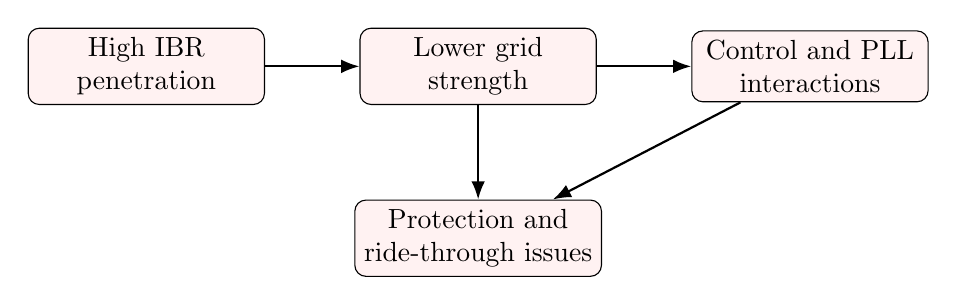
\begin{tikzpicture}[>=Latex,node distance=1.2cm]
  \tikzstyle{risk}=[draw,rounded corners,align=center,minimum width=3.0cm,minimum height=0.85cm,fill=red!5]
  \node[risk] (ibr) {High IBR\\penetration};
  \node[risk,right=of ibr] (strength) {Lower grid\\strength};
  \node[risk,right=of strength] (control) {Control and PLL\\interactions};
  \node[risk,below=of strength] (protect) {Protection and\\ride-through issues};
  \draw[->,thick] (ibr) -- (strength);
  \draw[->,thick] (strength) -- (control);
  \draw[->,thick] (strength) -- (protect);
  \draw[->,thick] (control) -- (protect);
\end{tikzpicture}
\caption{Main stability and protection concerns as IBR penetration increases.}
\end{figure}

\subsection{Microgrid Design Details}
A practical microgrid design should answer these questions:
\begin{enumerate}
  \item Which DER forms voltage and frequency when islanded?
  \item Is there enough spinning or synthetic reserve for the largest load step?
  \item Can the energy storage sustain islanded operation for the required time?
  \item Do protective devices detect faults in both grid-connected and islanded
  modes?
  \item How is the point of common coupling opened and resynchronized?
  \item Are black-start sequences defined and tested?
\end{enumerate}
For islanded power balance,
\begin{equation}
\sum P_{\mathrm{DER}}-\sum P_{\mathrm{load}}-P_{\mathrm{loss}}
=2H_{\mathrm{eq}}\omega\frac{\dd \omega}{\dd t}.
\end{equation}
In an inverter-only microgrid, $H_{\mathrm{eq}}$ is a control parameter rather
than physical inertia, and energy must still come from dc sources or storage.

\subsection{Fault Ride-Through: Detailed Control Logic}
The ride-through controller can be represented as a state machine:
\begin{center}
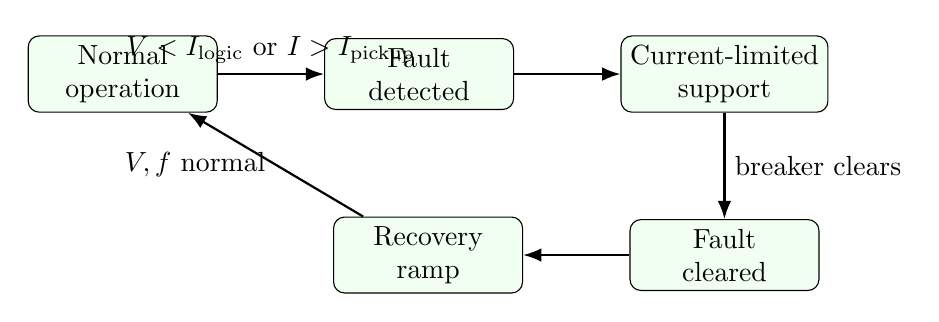
\begin{tikzpicture}[>=Latex,node distance=1.35cm]
  \tikzstyle{state}=[draw,rounded corners,align=center,minimum width=2.4cm,minimum height=0.8cm,fill=green!6]
  \node[state] (normal) {Normal\\operation};
  \node[state,right=of normal] (fault) {Fault\\detected};
  \node[state,right=of fault] (limit) {Current-limited\\support};
  \node[state,below=of limit] (clear) {Fault\\cleared};
  \node[state,left=of clear] (recover) {Recovery\\ramp};
  \draw[->,thick] (normal) -- node[above] {$V<I_{\mathrm{logic}}$ or $I>I_{\mathrm{pickup}}$} (fault);
  \draw[->,thick] (fault) -- (limit);
  \draw[->,thick] (limit) -- node[right] {breaker clears} (clear);
  \draw[->,thick] (clear) -- (recover);
  \draw[->,thick] (recover) -- node[left] {$V,f$ normal} (normal);
\end{tikzpicture}
\end{center}
In each state, limits must be explicit:
\begin{align}
|I|&\le I_{\max},\\
V_{\mathrm{dc,min}}&\le V_{\mathrm{dc}}\le V_{\mathrm{dc,max}},\\
T_{\mathrm{device}}&\le T_{\max},\\
\left|\frac{\dd i^*}{\dd t}\right|&\le r_i.
\end{align}

\paragraph{Why ride-through is hard in a microgrid.}
The same inverter may be responsible for voltage formation, fault current,
frequency regulation, and energy balancing. During a severe fault, these goals
conflict. A useful priority order is:
\begin{equation}
\text{device protection} > \text{safety/protection coordination} >
\text{voltage support} > \text{active-power delivery}.
\end{equation}

\subsection{Model Validation and Study Checklist}
For real projects, a study should document:
\begin{itemize}
  \item base cases, contingencies, and operating conditions,
  \item model source and validation status,
  \item protection settings and breaker clearing times,
  \item inverter current limits and control modes,
  \item voltage/frequency ride-through curves,
  \item load composition, especially motors and power-electronic loads,
  \item grid strength metrics at each interconnection point,
  \item sensitivity studies for dispatch, topology, and controller gains.
\end{itemize}

\section{Common Exam and Interview Questions}

\begin{enumerate}
  \item Why is one bus chosen as slack in power flow?
  \item What happens when a PV bus reaches reactive power limits?
  \item Why does $P$ mostly depend on angle and $Q$ mostly on voltage in a
  transmission grid?
  \item How do IBR fault currents differ from synchronous-generator fault currents?
  \item Why can a PLL destabilize a GFL inverter in a weak grid?
  \item What makes a GFM inverter useful for an islanded microgrid?
  \item How is low-voltage ride-through achieved without damaging the converter?
  \item Why can high IBR penetration require EMT instead of only RMS simulation?
  \item How do virtual impedance and current limiting help GFM fault ride-through?
  \item What protection functions remain dependable when fault current is low?
\end{enumerate}

\section{Quick Reference}

\begin{multicols}{2}
\subsection*{Essential Equations}
\begin{align*}
S &= VI^* = P+\junit Q\\
Z_{\mathrm{base}} &= V_{\mathrm{base}}^2/S_{\mathrm{base}}\\
I &= Y_{\mathrm{bus}}V\\
P_i &= |V_i|\sum_k |V_k|(G_{ik}\cos\delta_{ik}+B_{ik}\sin\delta_{ik})\\
Q_i &= |V_i|\sum_k |V_k|(G_{ik}\sin\delta_{ik}-B_{ik}\cos\delta_{ik})\\
P_e &= \frac{EV}{X}\sin\delta\\
2H\dot{\omega} &= P_m-P_e-D(\omega-\omega_0)\\
\mathrm{SCR} &= S_{\mathrm{sc}}/S_{\mathrm{IBR,rated}}\\
I_{\mathrm{IBR}} &\le I_{\max}
\end{align*}

\subsection*{Study Priorities}
\begin{itemize}[leftmargin=*]
  \item Know bus types and power-flow equations.
  \item Understand voltage, angle, and frequency stability separately.
  \item Compare SG and IBR fault behavior.
  \item Distinguish GFL current-source behavior from GFM voltage-source behavior.
  \item For microgrids, connect controls, energy balance, and protection.
\end{itemize}
\end{multicols}

\section{Suggested Learning Path}
\begin{enumerate}
  \item Review phasors, complex power, and per-unit calculations.
  \item Build $Y_{\mathrm{bus}}$ for a three-bus system and solve power flow.
  \item Study symmetrical components and compute SLG and three-phase faults.
  \item Simulate swing-equation response to a generation trip.
  \item Compare GFL and GFM inverter block diagrams and control equations.
  \item Analyze how current limits alter fault response and voltage support.
  \item Study a microgrid fault sequence: detect, limit, support, isolate, recover.
  \item Move from RMS to EMT simulation when converter controls dominate dynamics.
\end{enumerate}

\end{document}
